% Options for packages loaded elsewhere
\PassOptionsToPackage{unicode}{hyperref}
\PassOptionsToPackage{hyphens}{url}
\PassOptionsToPackage{dvipsnames,svgnames,x11names}{xcolor}
%
\documentclass[
  letterpaper,
  DIV=11,
  numbers=noendperiod]{scrartcl}

\usepackage{amsmath,amssymb}
\usepackage{lmodern}
\usepackage{iftex}
\ifPDFTeX
  \usepackage[T1]{fontenc}
  \usepackage[utf8]{inputenc}
  \usepackage{textcomp} % provide euro and other symbols
\else % if luatex or xetex
  \usepackage{unicode-math}
  \defaultfontfeatures{Scale=MatchLowercase}
  \defaultfontfeatures[\rmfamily]{Ligatures=TeX,Scale=1}
\fi
% Use upquote if available, for straight quotes in verbatim environments
\IfFileExists{upquote.sty}{\usepackage{upquote}}{}
\IfFileExists{microtype.sty}{% use microtype if available
  \usepackage[]{microtype}
  \UseMicrotypeSet[protrusion]{basicmath} % disable protrusion for tt fonts
}{}
\makeatletter
\@ifundefined{KOMAClassName}{% if non-KOMA class
  \IfFileExists{parskip.sty}{%
    \usepackage{parskip}
  }{% else
    \setlength{\parindent}{0pt}
    \setlength{\parskip}{6pt plus 2pt minus 1pt}}
}{% if KOMA class
  \KOMAoptions{parskip=half}}
\makeatother
\usepackage{xcolor}
\setlength{\emergencystretch}{3em} % prevent overfull lines
\setcounter{secnumdepth}{5}
% Make \paragraph and \subparagraph free-standing
\ifx\paragraph\undefined\else
  \let\oldparagraph\paragraph
  \renewcommand{\paragraph}[1]{\oldparagraph{#1}\mbox{}}
\fi
\ifx\subparagraph\undefined\else
  \let\oldsubparagraph\subparagraph
  \renewcommand{\subparagraph}[1]{\oldsubparagraph{#1}\mbox{}}
\fi


\providecommand{\tightlist}{%
  \setlength{\itemsep}{0pt}\setlength{\parskip}{0pt}}\usepackage{longtable,booktabs,array}
\usepackage{calc} % for calculating minipage widths
% Correct order of tables after \paragraph or \subparagraph
\usepackage{etoolbox}
\makeatletter
\patchcmd\longtable{\par}{\if@noskipsec\mbox{}\fi\par}{}{}
\makeatother
% Allow footnotes in longtable head/foot
\IfFileExists{footnotehyper.sty}{\usepackage{footnotehyper}}{\usepackage{footnote}}
\makesavenoteenv{longtable}
\usepackage{graphicx}
\makeatletter
\def\maxwidth{\ifdim\Gin@nat@width>\linewidth\linewidth\else\Gin@nat@width\fi}
\def\maxheight{\ifdim\Gin@nat@height>\textheight\textheight\else\Gin@nat@height\fi}
\makeatother
% Scale images if necessary, so that they will not overflow the page
% margins by default, and it is still possible to overwrite the defaults
% using explicit options in \includegraphics[width, height, ...]{}
\setkeys{Gin}{width=\maxwidth,height=\maxheight,keepaspectratio}
% Set default figure placement to htbp
\makeatletter
\def\fps@figure{htbp}
\makeatother
\newlength{\cslhangindent}
\setlength{\cslhangindent}{1.5em}
\newlength{\csllabelwidth}
\setlength{\csllabelwidth}{3em}
\newlength{\cslentryspacingunit} % times entry-spacing
\setlength{\cslentryspacingunit}{\parskip}
\newenvironment{CSLReferences}[2] % #1 hanging-ident, #2 entry spacing
 {% don't indent paragraphs
  \setlength{\parindent}{0pt}
  % turn on hanging indent if param 1 is 1
  \ifodd #1
  \let\oldpar\par
  \def\par{\hangindent=\cslhangindent\oldpar}
  \fi
  % set entry spacing
  \setlength{\parskip}{#2\cslentryspacingunit}
 }%
 {}
\usepackage{calc}
\newcommand{\CSLBlock}[1]{#1\hfill\break}
\newcommand{\CSLLeftMargin}[1]{\parbox[t]{\csllabelwidth}{#1}}
\newcommand{\CSLRightInline}[1]{\parbox[t]{\linewidth - \csllabelwidth}{#1}\break}
\newcommand{\CSLIndent}[1]{\hspace{\cslhangindent}#1}

\KOMAoption{captions}{tableheading}
\makeatletter
\makeatother
\makeatletter
\makeatother
\makeatletter
\@ifpackageloaded{caption}{}{\usepackage{caption}}
\AtBeginDocument{%
\ifdefined\contentsname
  \renewcommand*\contentsname{Table of contents}
\else
  \newcommand\contentsname{Table of contents}
\fi
\ifdefined\listfigurename
  \renewcommand*\listfigurename{List of Figures}
\else
  \newcommand\listfigurename{List of Figures}
\fi
\ifdefined\listtablename
  \renewcommand*\listtablename{List of Tables}
\else
  \newcommand\listtablename{List of Tables}
\fi
\ifdefined\figurename
  \renewcommand*\figurename{Figure}
\else
  \newcommand\figurename{Figure}
\fi
\ifdefined\tablename
  \renewcommand*\tablename{Table}
\else
  \newcommand\tablename{Table}
\fi
}
\@ifpackageloaded{float}{}{\usepackage{float}}
\floatstyle{ruled}
\@ifundefined{c@chapter}{\newfloat{codelisting}{h}{lop}}{\newfloat{codelisting}{h}{lop}[chapter]}
\floatname{codelisting}{Listing}
\newcommand*\listoflistings{\listof{codelisting}{List of Listings}}
\makeatother
\makeatletter
\@ifpackageloaded{caption}{}{\usepackage{caption}}
\@ifpackageloaded{subcaption}{}{\usepackage{subcaption}}
\makeatother
\makeatletter
\@ifpackageloaded{tcolorbox}{}{\usepackage[many]{tcolorbox}}
\makeatother
\makeatletter
\@ifundefined{shadecolor}{\definecolor{shadecolor}{rgb}{.97, .97, .97}}
\makeatother
\makeatletter
\makeatother
\ifLuaTeX
  \usepackage{selnolig}  % disable illegal ligatures
\fi
\IfFileExists{bookmark.sty}{\usepackage{bookmark}}{\usepackage{hyperref}}
\IfFileExists{xurl.sty}{\usepackage{xurl}}{} % add URL line breaks if available
\urlstyle{same} % disable monospaced font for URLs
\hypersetup{
  pdftitle={Supplement to Example Manuscript Template for a Data Analysis Project},
  pdfauthor={Andreas Handel},
  colorlinks=true,
  linkcolor={blue},
  filecolor={Maroon},
  citecolor={Blue},
  urlcolor={Blue},
  pdfcreator={LaTeX via pandoc}}

\title{Supplement to Example Manuscript Template for a Data Analysis
Project}
\author{Andreas Handel}
\date{2/2/23}

\begin{document}
\maketitle
\ifdefined\Shaded\renewenvironment{Shaded}{\begin{tcolorbox}[borderline west={3pt}{0pt}{shadecolor}, boxrule=0pt, sharp corners, interior hidden, enhanced, breakable, frame hidden]}{\end{tcolorbox}}\fi

This shows some materials that could go into a supplementary file. Often
you want/need references here too. You can use the same reference bib
file for this and the main text (as done here) or have separate bib
files.

For illustrative purposes, I'm doing the supplement as pdf. For this to
work, you need a (La)TeX system installed. It's easy. Just follow
\href{https://quarto.org/docs/output-formats/pdf-basics.html}{these
steps}.

Of course you would choose the format based on needs.

I'm also using a different style for the references here. (vancouver vs
apa in the main manuscript). Usually one would have the formatting of
the references the same in those two documents, but I want to illustrate
how easy it is to switch reference formatting styles, you just need to
get the right CSL file and specify it in the YAML header. We could also
have a seperate reference bibtext (\texttt{.bib}) file, but here we are
using the same.

\hypertarget{overview}{%
\section{Overview}\label{overview}}

A quick overview of what readers can find in the supplement.

\hypertarget{code-and-file-information}{%
\section{Code and file information}\label{code-and-file-information}}

Explain here what each code/file is and does, and in which order (if
any) users need to run thing to reproduce everything. Essentially, give
a full set of instructions to re-generate everything.

\newpage{}

\hypertarget{additional-method-details}{%
\section{Additional Method Details}\label{additional-method-details}}

Often, the main manuscript only allows for an overview description of
the methods. Use the supplement to describe all your methods, models and
approaches in a lot of detail. Reference specific parts of your code as
needed.

\newpage{}

\hypertarget{additional-results}{%
\section{Additional results}\label{additional-results}}

Show additional results here. Those can be some useful
exploratory/descriptive figures or tables, or results from additional
analyses that didn't make it into the main text.

\hypertarget{example-additional-result}{%
\subsection{Example additional result}\label{example-additional-result}}

Table~\ref{tbl-resulttable1} shows an additional table summarizing a
model fit.

\hypertarget{tbl-resulttable1}{}
\begin{longtable}[]{@{}lrrrr@{}}
\caption{\label{tbl-resulttable1}Another fit table.}\tabularnewline
\toprule()
term & estimate & std.error & statistic & p.value \\
\midrule()
\endfirsthead
\toprule()
term & estimate & std.error & statistic & p.value \\
\midrule()
\endhead
(Intercept) & 149.6997661 & 19.7518528 & 7.5790240 & 0.0001285 \\
Weight & 0.2277371 & 0.2708841 & 0.8407177 & 0.4282860 \\
\bottomrule()
\end{longtable}

Figure~\ref{fig-result2} shows a scatterplot figure produced by one of
the R scripts.

\begin{figure}

{\centering 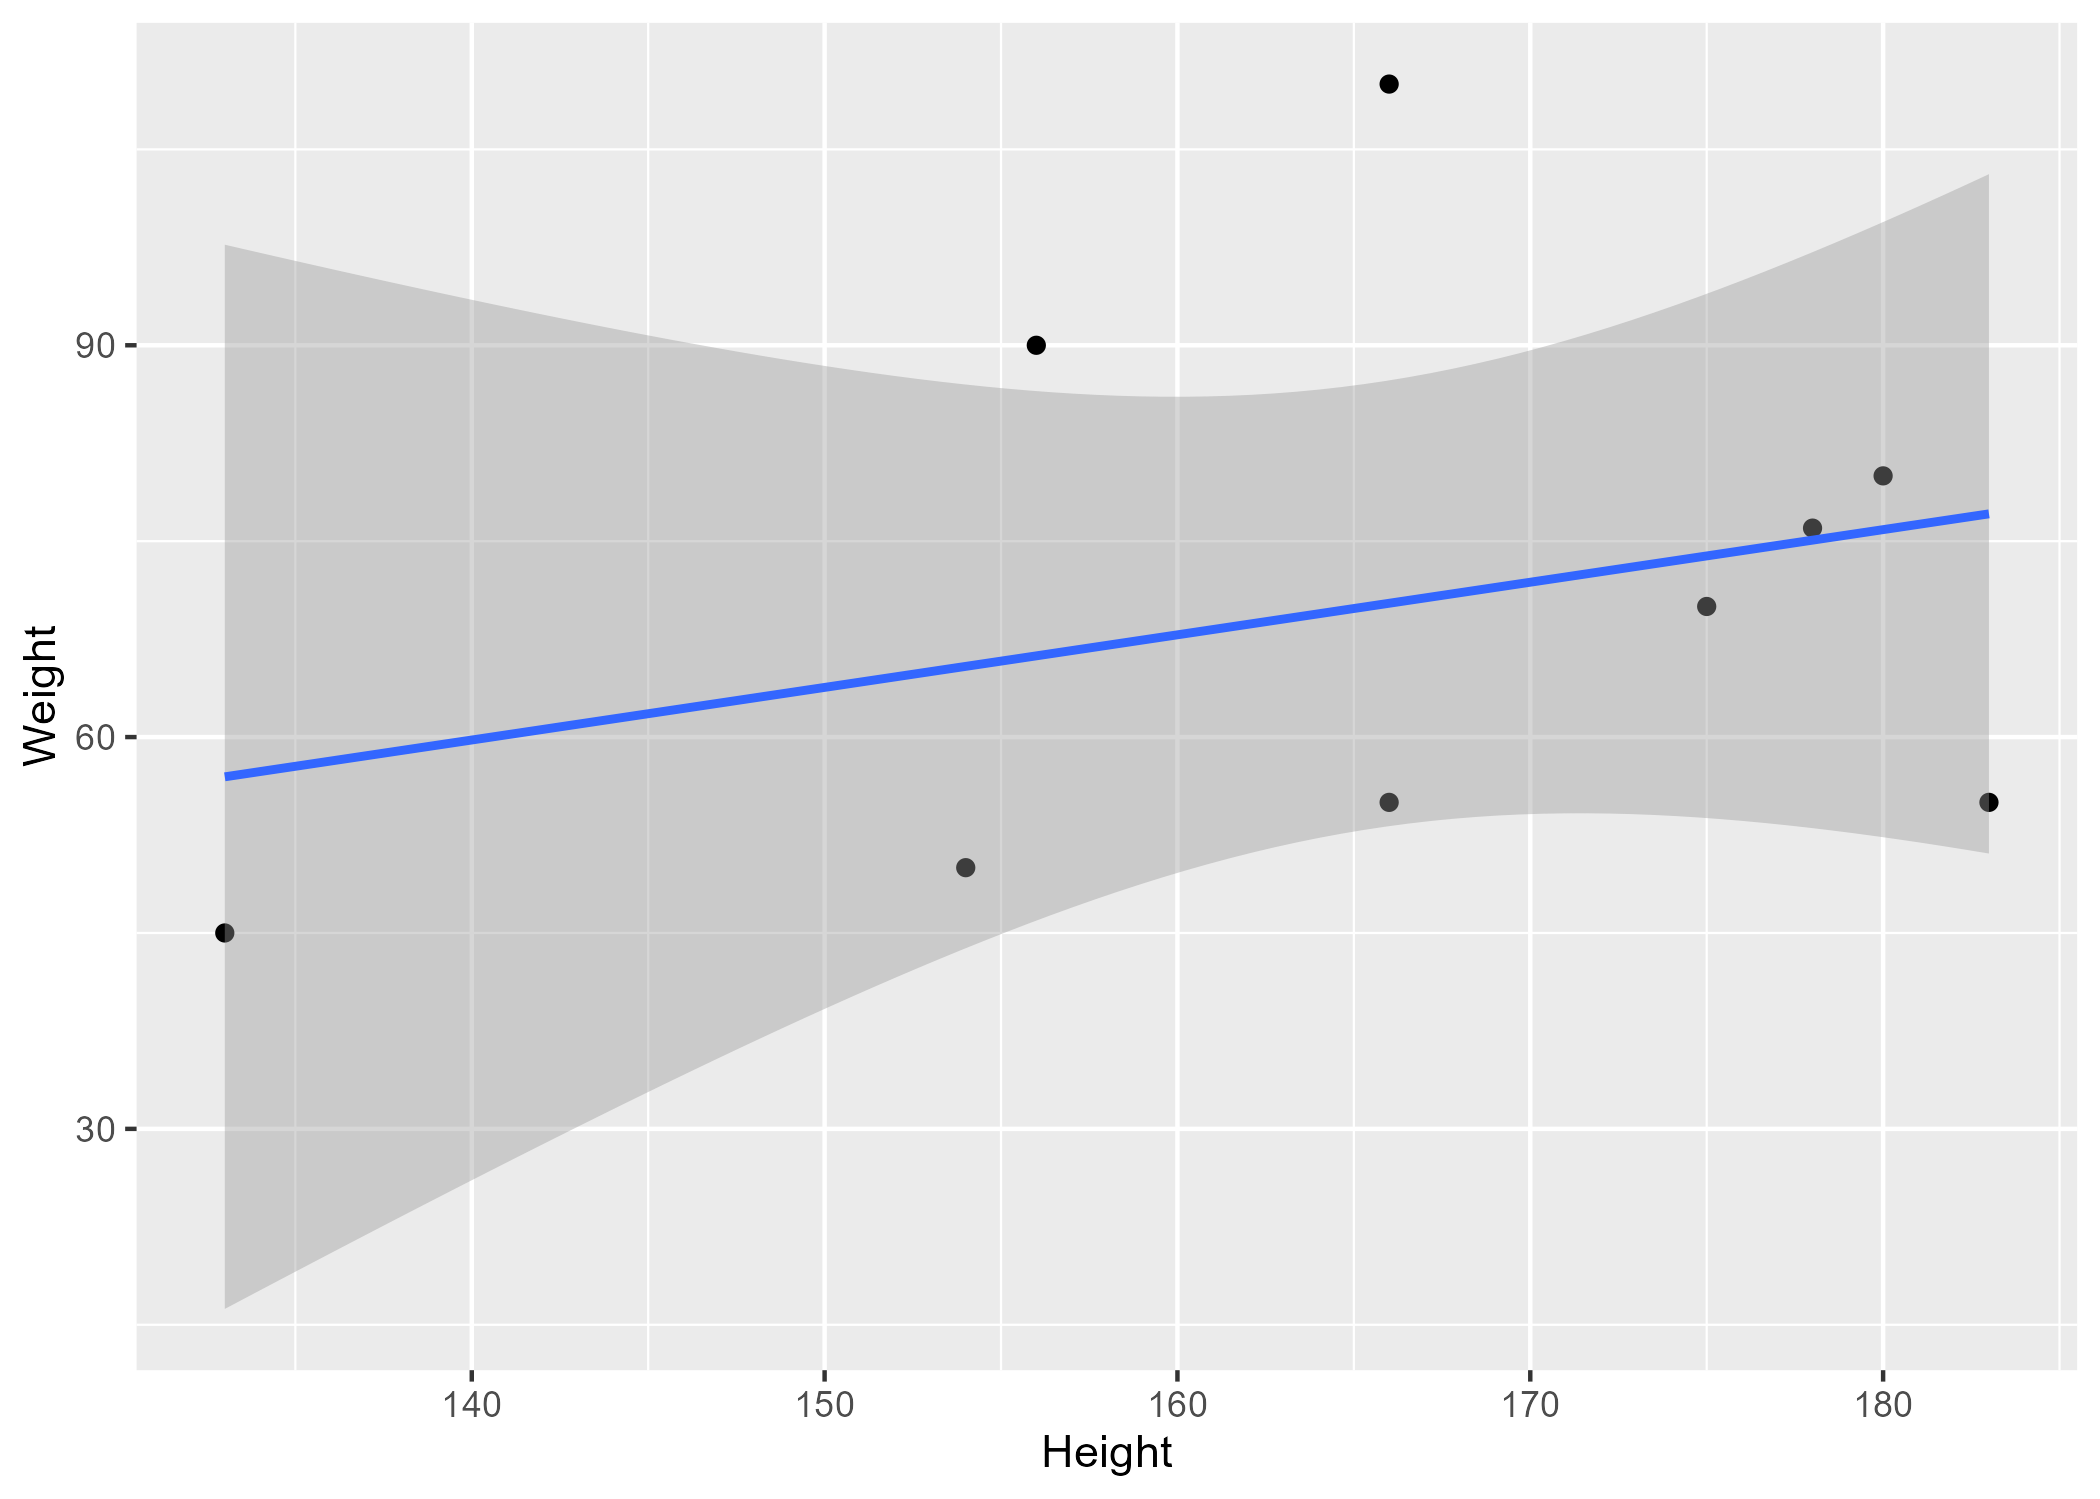
\includegraphics[width=7in,height=\textheight]{../../../results/height_weight.png}

}

\caption{\label{fig-result2}Height and weight.}

\end{figure}

\newpage{}

\hypertarget{discussion}{%
\section{Discussion}\label{discussion}}

Any additional discussion regarding the supplementary material/findings.

These papers (1,2) are good examples of papers published using a fully
reproducible setup similar to the one shown in this template.

\newpage{}

\hypertarget{references}{%
\section*{References}\label{references}}
\addcontentsline{toc}{section}{References}

\hypertarget{refs}{}
\begin{CSLReferences}{0}{0}
\leavevmode\vadjust pre{\hypertarget{ref-mckay2020}{}}%
\CSLLeftMargin{1. }%
\CSLRightInline{McKay B, Ebell M, Billings WZ, Dale AP, Shen Y, Handel
A. \href{https://doi.org/10.1093/ofid/ofaa494}{Associations {Between
Relative Viral Load} at {Diagnosis} and {Influenza A Symptoms} and
{Recovery}.} Open forum infectious diseases. 2020 Nov;7(11):ofaa494. }

\leavevmode\vadjust pre{\hypertarget{ref-mckay2020a}{}}%
\CSLLeftMargin{2. }%
\CSLRightInline{McKay B, Ebell M, Dale AP, Shen Y, Handel A.
\href{https://doi.org/10.1098/rspb.2020.0496}{Virulence-mediated
infectiousness and activity trade-offs and their impact on transmission
potential of influenza patients.} Proceedings Biological sciences. 2020
May;287(1927):20200496. }

\end{CSLReferences}



\end{document}
